\section{Principe général}
L'objectif de ce laboratoire est d'utiliser l'ADC que contient le PIC18F et de convertir la tension d'entrée en une valeur numérique codée sur 10 bits et stockée dans une variable de 16 bits. Il sera donc important de spécifier si l'on désire aligner nos bits à gauche ou à droite.(cf FIG \ref{align})

\begin{figure}
\begin{center}
\begin{framed}
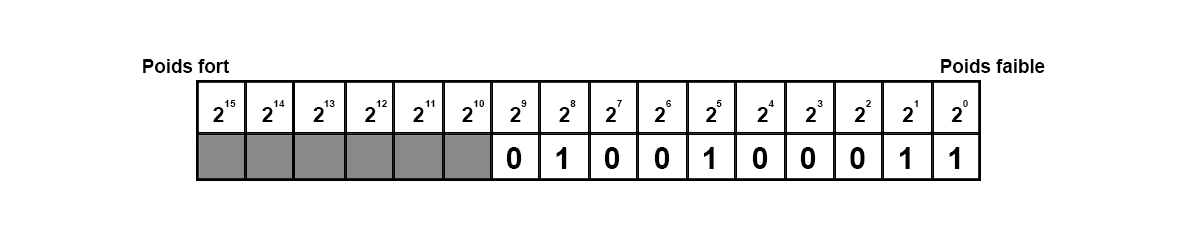
\includegraphics[scale=0.8]{images/aligndroite.png}
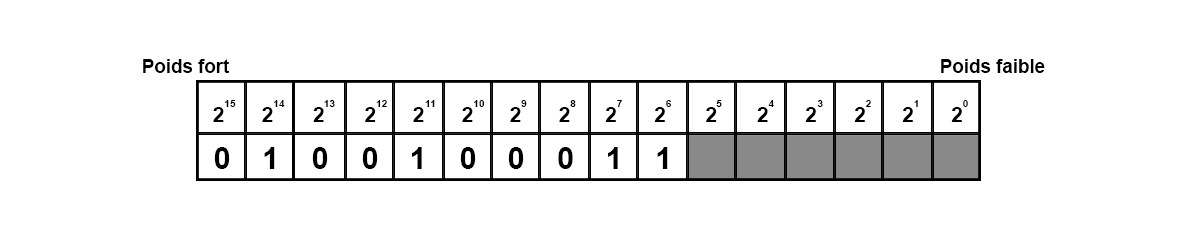
\includegraphics[scale=0.8]{images/aligngauche.png}
\caption{Alignement des 10 bits encodés dans la variable sur 16 bits}
\label{align}
\end{framed}
\end{center}
\end{figure}

\subsection{Paramètres de l'ADC}

\subsubsection*{Tensions de références}
Bornes de tension entre lesquelles le PIC18F convertira le signal d'entrée. Si la tension mesurée se situe entre les deux bornes, alors la valeur digitale retournée sera calculée proportionnellement aux valeurs binaires extrêmes.(Dans ce laboratoire nous choisirons $V_{SS}$ et $V_{DD}$ comme tensions de références basse et haute)
\subsubsection*{Temps de conversion Analogique $\rightarrow$ Digital  ($T_{AD}$)}
Le $T_{AD}$  est le temps minimum nécessaire à l'ADC pour mesurer un bit. Le $T_{AD}$ se configure comme un multiple en puissance de 2 de la période d'oscillation de la clock du PIC18F ($T_{osc} = 25ns$).
\subsubsection*{Temps d'acquisition ($T_{ACQ}$)}
Le $T_{ACQ}$ est le temps minimum nécessaire pour que le condensateur CHOLD se charge. Le $T_{ACQ}$  se configure comme un multiple de 2 du $T_{AD}$. 
 